

\tikzset{every picture/.style={line width=0.75pt}} %set default line width to 0.75pt        

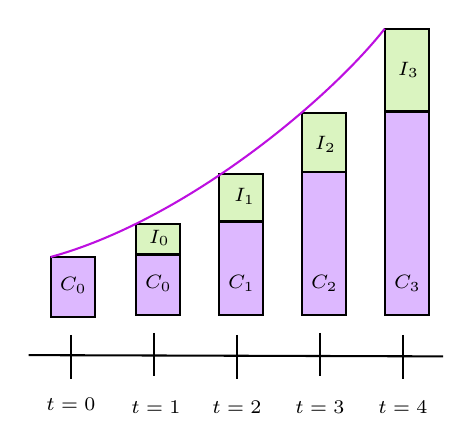
\begin{tikzpicture}[x=0.75pt,y=0.75pt,yscale=-1,xscale=1]
%uncomment if require: \path (0,300); %set diagram left start at 0, and has height of 300

%Straight Lines [id:da30833855228946516] 
\draw    (203,197) -- (402.68,197.61) ;
%Shape: Rectangle [id:dp9691673674813379] 
\draw  [fill={rgb, 255:red, 144; green, 19; blue, 254 }  ,fill opacity=0.3 ] (213.53,149.73) -- (234.81,149.73) -- (234.81,178.73) -- (213.53,178.73) -- cycle ;
%Straight Lines [id:da06693566861753752] 
\draw    (223.2,187.27) -- (223.2,208.27) ;
%Straight Lines [id:da21764506729039024] 
\draw    (263.2,186.27) -- (263.2,207.27) ;
%Shape: Rectangle [id:dp05878456747808403] 
\draw  [fill={rgb, 255:red, 184; green, 233; blue, 134 }  ,fill opacity=0.52 ] (254.53,133.8) -- (275.81,133.8) -- (275.81,148.53) -- (254.53,148.53) -- cycle ;
%Straight Lines [id:da45506013679394786] 
\draw    (303.2,187.27) -- (303.2,208.27) ;
%Straight Lines [id:da4961958798357171] 
\draw    (343.2,186.27) -- (343.2,207.27) ;
%Straight Lines [id:da7612017790642615] 
\draw    (383.2,187.27) -- (383.2,208.27) ;
%Shape: Rectangle [id:dp009455518583604605] 
\draw  [fill={rgb, 255:red, 144; green, 19; blue, 254 }  ,fill opacity=0.3 ] (254.53,148.73) -- (275.81,148.73) -- (275.81,177.73) -- (254.53,177.73) -- cycle ;
%Shape: Rectangle [id:dp5087701140221421] 
\draw  [fill={rgb, 255:red, 144; green, 19; blue, 254 }  ,fill opacity=0.3 ] (294.53,132.73) -- (315.81,132.73) -- (315.81,177.73) -- (294.53,177.73) -- cycle ;
%Shape: Rectangle [id:dp1417867858106694] 
\draw  [fill={rgb, 255:red, 184; green, 233; blue, 134 }  ,fill opacity=0.52 ] (294.53,109.73) -- (315.81,109.73) -- (315.81,132.53) -- (294.53,132.53) -- cycle ;
%Shape: Rectangle [id:dp018590783147910517] 
\draw  [fill={rgb, 255:red, 144; green, 19; blue, 254 }  ,fill opacity=0.3 ] (334.53,108.97) -- (355.81,108.97) -- (355.81,177.73) -- (334.53,177.73) -- cycle ;
%Shape: Rectangle [id:dp22782483522166164] 
\draw  [fill={rgb, 255:red, 184; green, 233; blue, 134 }  ,fill opacity=0.52 ] (334.53,80.41) -- (355.81,80.41) -- (355.81,108.97) -- (334.53,108.97) -- cycle ;
%Shape: Rectangle [id:dp6637335203221238] 
\draw  [fill={rgb, 255:red, 144; green, 19; blue, 254 }  ,fill opacity=0.3 ] (374.53,79.97) -- (395.81,79.97) -- (395.81,177.73) -- (374.53,177.73) -- cycle ;
%Shape: Rectangle [id:dp5353689255714892] 
\draw  [fill={rgb, 255:red, 184; green, 233; blue, 134 }  ,fill opacity=0.52 ] (374.53,39.74) -- (395.81,39.74) -- (395.81,79.53) -- (374.53,79.53) -- cycle ;
%Curve Lines [id:da16909378811175346] 
\draw [color={rgb, 255:red, 189; green, 16; blue, 224 }  ,draw opacity=1 ]   (213.53,149.73) .. controls (278.66,131.85) and (347.66,73.85) .. (374.53,39.74) ;

% Text Node
\draw (210,216.4) node [anchor=north west][inner sep=0.75pt]  [font=\scriptsize]  {${\textstyle t=0}$};
% Text Node
\draw (251,217.4) node [anchor=north west][inner sep=0.75pt]  [font=\scriptsize]  {$t=1$};
% Text Node
\draw (290,217.4) node [anchor=north west][inner sep=0.75pt]  [font=\scriptsize]  {$t=2$};
% Text Node
\draw (330,217.4) node [anchor=north west][inner sep=0.75pt]  [font=\scriptsize]  {$t=3$};
% Text Node
\draw (370,217.4) node [anchor=north west][inner sep=0.75pt]  [font=\scriptsize]  {$t=4$};
% Text Node
\draw (216.53,157.93) node [anchor=north west][inner sep=0.75pt]  [font=\scriptsize]  {$C_{0}$};
% Text Node
\draw (259.53,135.13) node [anchor=north west][inner sep=0.75pt]  [font=\scriptsize]  {$I_{0}$};
% Text Node
\draw (257.53,156.93) node [anchor=north west][inner sep=0.75pt]  [font=\scriptsize]  {$C_{0}$};
% Text Node
\draw (297.53,156.93) node [anchor=north west][inner sep=0.75pt]  [font=\scriptsize]  {$C_{1}$};
% Text Node
\draw (300.53,115.13) node [anchor=north west][inner sep=0.75pt]  [font=\scriptsize]  {$I_{1}$};
% Text Node
\draw (337.53,156.93) node [anchor=north west][inner sep=0.75pt]  [font=\scriptsize]  {$C_{2}$};
% Text Node
\draw (339.53,90.13) node [anchor=north west][inner sep=0.75pt]  [font=\scriptsize]  {$I_{2}$};
% Text Node
\draw (377.53,156.93) node [anchor=north west][inner sep=0.75pt]  [font=\scriptsize]  {$C_{3}$};
% Text Node
\draw (379.53,54.17) node [anchor=north west][inner sep=0.75pt]  [font=\scriptsize]  {$I_{3}$};


\end{tikzpicture}